\section{System Design Overview}
{\fontsize{12}{14}\selectfont
    The smart water level monitoring system consists of sensors, microcontrollers, and IoT technology for efficient and automated water management. Below is an overview of the system design: \\
    
    \begin{enumerate}
    \item \textbf{Components and Hardware Design}
    \begin{itemize}
        \item \textbf{Ultrasonic Sensor (HC-SR04)}: Measures the distance to the water surface and determines the water level.
        \item \textbf{Microcontroller (NodeMCU or Raspberry Pi)}: Processes sensor data, controls pump operations, and connects to the Blynk cloud.
        \item \textbf{Wi-Fi Module (Built-in NodeMCU)}: Allows for remote monitoring and real-time feedback from the Blynk application.
        \item \textbf{OLED Display (0.96-inch)}: Visualizes water levels locally.
        \item \textbf{Buzzer}: Signals over/underflow or low level.
        \item \textbf{Water Pump}: Controlled automatically with preset water level thresholds.
        \item \textbf{Power Supply}: Stabilizes all elements to ensure continuous running of the system.
    \end{itemize}
    
    \item \textbf{Functional Modules}
    \begin{itemize}
        \item \textbf{Data Acquisition Module:}  
        The ultrasonic sensor captures water level information based on the distance from the surface.
        \item \textbf{Processing Module:}  
        Microcontroller processes sensor inputs, determining whether alerts are required or the pump should be switched on.
        \item \textbf{Communication Module:}  
        Wi-Fi ensures that all data is uploaded to the Blynk cloud, thereby providing remote access and control.
        \item \textbf{Display Module:}  
        OLED Screen shows real-time information for water level information in local access.
        \item \textbf{Control Module:}  
        \begin{itemize}
            \item The automated pumping is controlled based on preset thresholds to maintain a target level of water.
            \item Override via the mobile application to make custom operations.
        \end{itemize}
    \end{itemize}

    \item \textbf{Software Design}
    \begin{itemize}
        \item \textbf{Blynk Integration:}  
        Real-time monitoring and control through the Blynk application, including notified alerts and notifications to the mobile.
        \item \textbf{Cloud Connectivity:}  
        Data can be saved in the Blynk cloud, visualized, and insights can be derived over history. The system automatically switches the pump ON or OFF based on the sensor readings to minimize manual intervention.
    \end{itemize}

    \item \textbf{Workflow}
    \begin{itemize}
        \item The ultrasonic sensor takes real-time measurements of the water level.
        \item Sensor data is transmitted to the microcontroller for processing.
        \item The microcontroller updates the OLED display and sends data to the Blynk cloud.
        \item Depending on the water level:
        \begin{itemize}
            \item If it is low, the pump is turned ON.
            \item If it is full, the pump is turned OFF.
        \end{itemize}
        \item Users are notified on their mobile devices through the Blynk app.
        \item Alerts are thrown if critical thresholds (overflow/low water) are exceeded.
    \end{itemize}

    \item \textbf{Scalability and Future Enhancements}
    \begin{itemize}
        \item Support for multiple tanks or reservoirs.
        \item Additional sensors that could be integrated for quality water monitoring, such as pH and turbidity.
        \item Further advanced data analysis and insights from cloud services.
        \item This design of the system will come in as cost-effective and scalable with reliability in providing real-time water level monitoring and resource management.
    \end{itemize}
\end{enumerate}

\section{Hardware Components Used}
\begin{enumerate}
    \item \textbf{Ultrasonic Sensor (HC-SR04)}\\
        \begin{figure}[H]
            \centering
            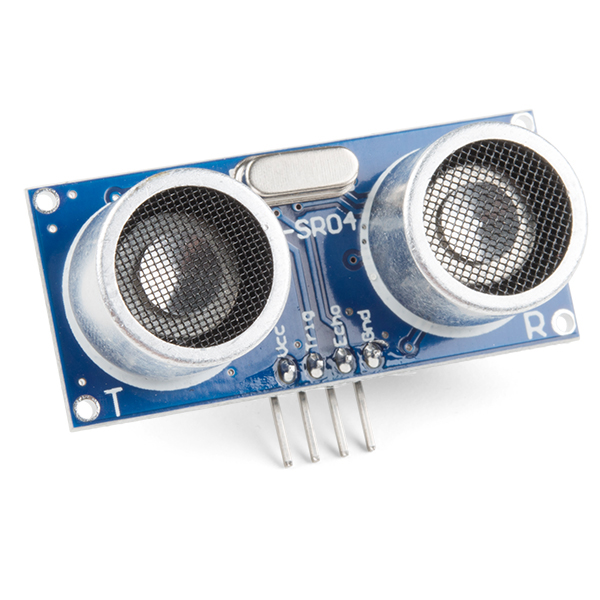
\includegraphics[width=1.75in]{ultrasonic.jpg} \\
            \caption{Ultrasonic Sensor (HC-SR04)}
            \label{fig:ultrasonic} % Optional: for referencing
        \end{figure}
    The HC-SR04 is a widely used ultrasonic sensor designed for distance measurement. It operates by emitting ultrasonic waves at a frequency of 40 kHz through its transmitter and receiving the echo reflected from an object via its receiver. The time taken for the echo to return is measured and used to calculate the distance to the object based on the speed of sound.
    
    \item \textbf{Microcontroller (NodeMCU/ESP8266)}\\
    \begin{figure}[H]
            \centering
            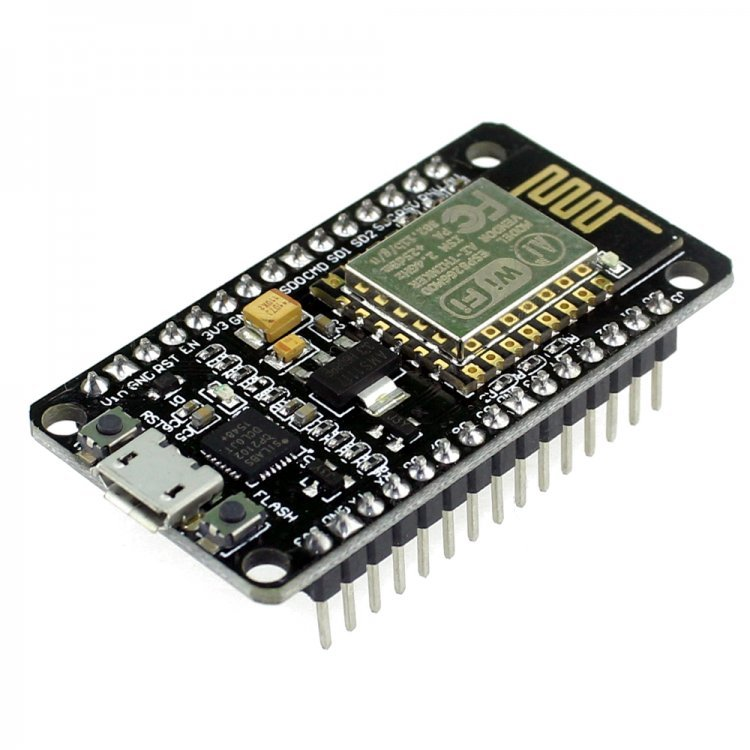
\includegraphics[width=1.75in]{esp.jpg} \\
            \caption{NodeMCU/ ESP8266}
            \label{fig:esp} % Optional: for referencing
        \end{figure}
    The ESP8266 is a low-cost Wi-Fi-enabled microcontroller that serves as the system's core processing unit. It processes data from sensors, executes control logic, and facilitates wireless communication with cloud platforms and mobile devices. Its built-in Wi-Fi module makes it ideal for IoT applications.

    
    \item \textbf{0.96'' OLED Display}\\
    \begin{figure}[H]
            \centering
            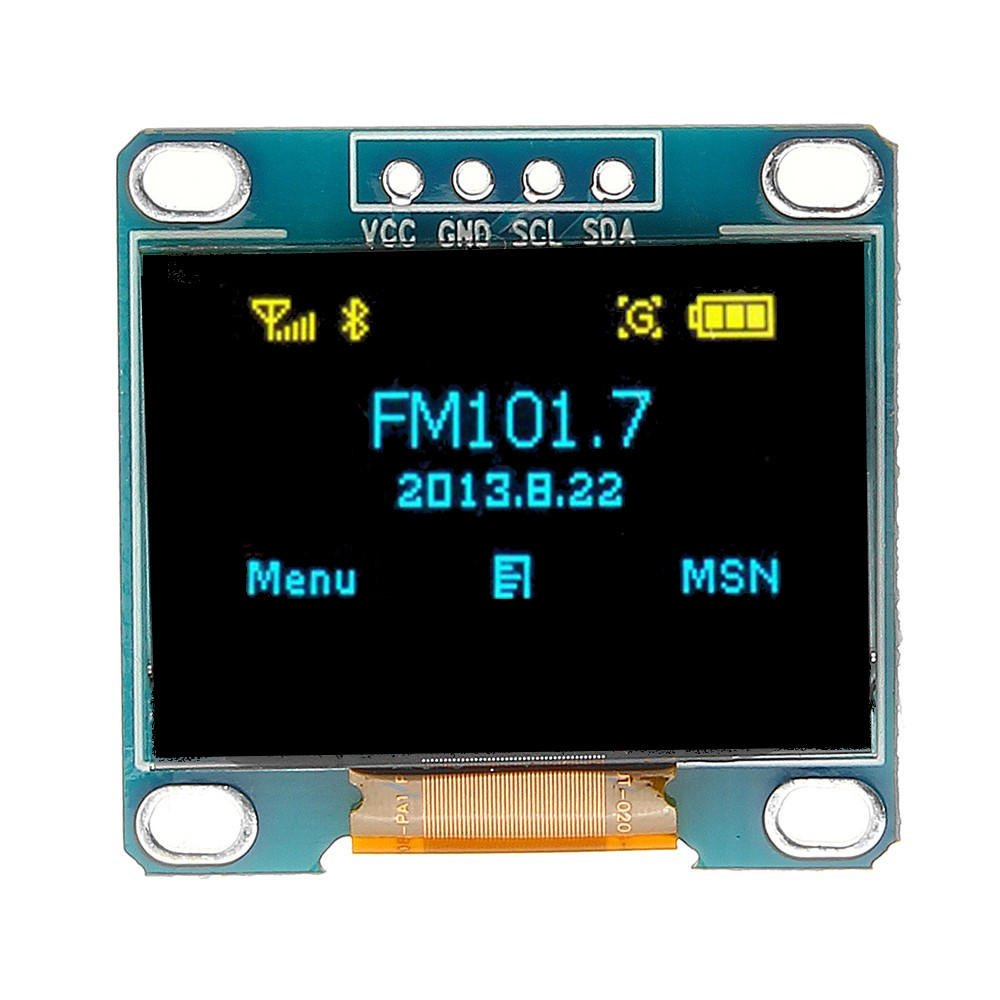
\includegraphics[width=1.75in]{oled.jpg} \\
            \caption{0.96''OLED Display}
            \label{fig:oled} % Optional: for referencing
        \end{figure}
    A 0.96-inch OLED display is a compact, high-contrast, and energy-efficient screen used in IoT projects to visually present data such as sensor readings, system status, or notifications.

    \item \textbf{Buzzer}\\
    \begin{figure}[H]
            \centering
            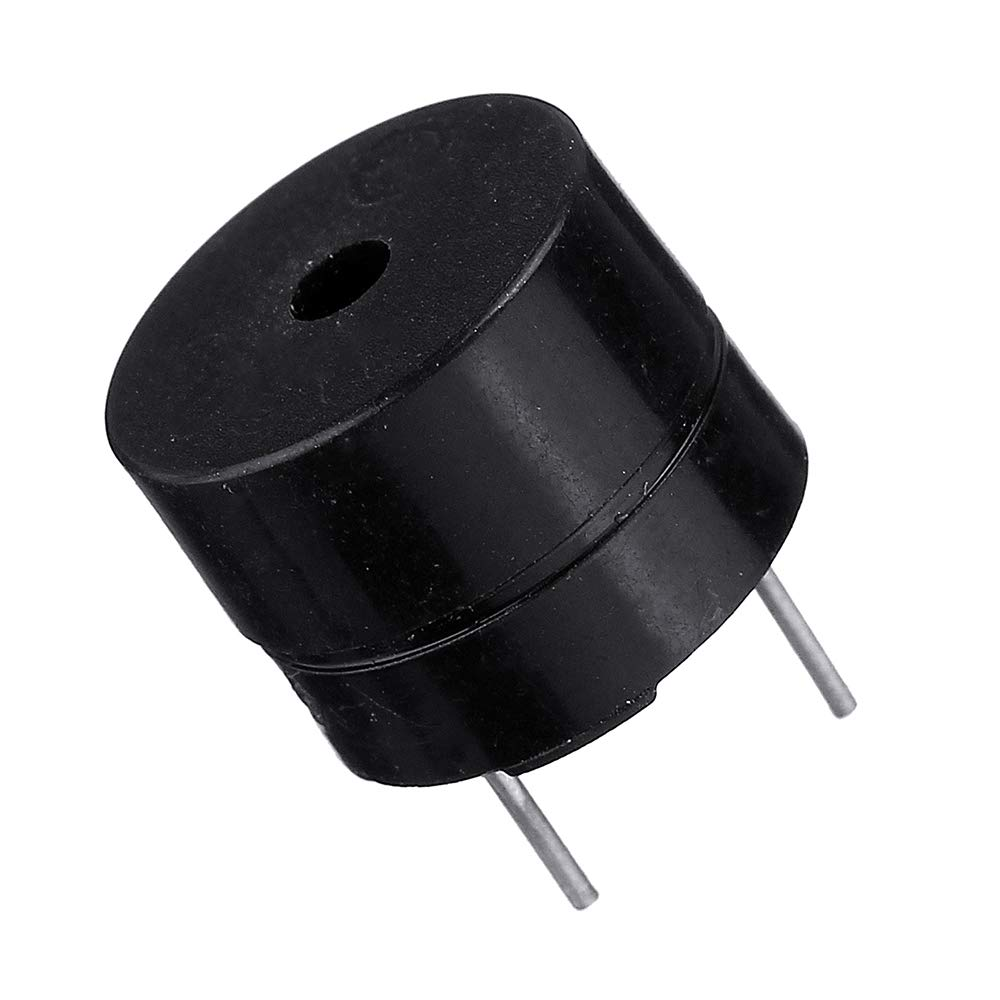
\includegraphics[width=1.75in]{buzzer.jpg} \\
            \caption{Buzzer}
            \label{fig:buzzer} % Optional: for referencing
        \end{figure}
    An electronic signaling device that produces sound. Commonly used in alarms, timers, and notifications in electronic circuits.
    
    \item \textbf{Push Buttons}\\
    \begin{figure}[H]
            \centering
            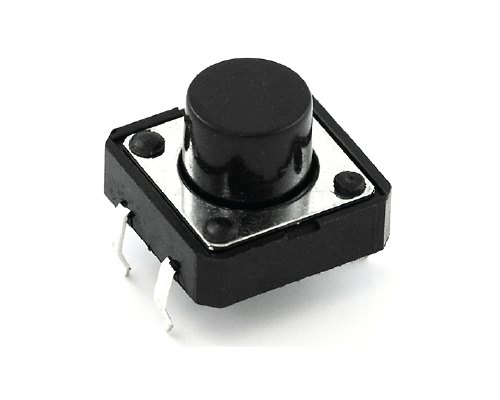
\includegraphics[width=1.75in]{push.png} \\
            \caption{Push Button}
            \label{fig:push-button} % Optional: for referencing
        \end{figure}
    Push button is a basic input device used in electronic and IoT projects to make or break a circuit connection when pressed. It has two terminals (pins) and functions as a single-pole, single-throw (SPST) switch, offering a simple way to send a digital signal to the microcontroller.
    
    \item \textbf{Jumper Wires}\\
    \begin{figure}[H]
            \centering
            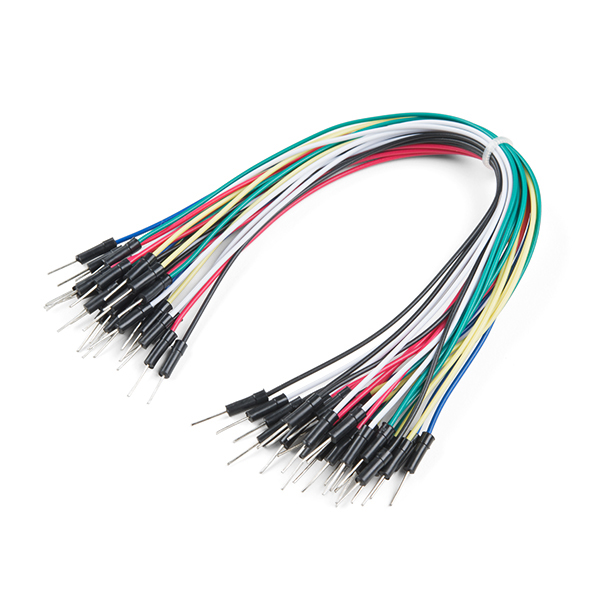
\includegraphics[width=1.75in]{jumper-wire.jpg} \\
            \caption{Jumper Wires}
            \label{fig:jumper-wire} 
        \end{figure}
    Short wires with connectors at each end, used to create temporary electrical connections on breadboards or between components. Facilitates quick and flexible connections in prototyping and troubleshooting electronic circuits.
    
    \item \textbf{AC to DC Converter (Relay)}\\
    \begin{figure}[H]
            \centering
            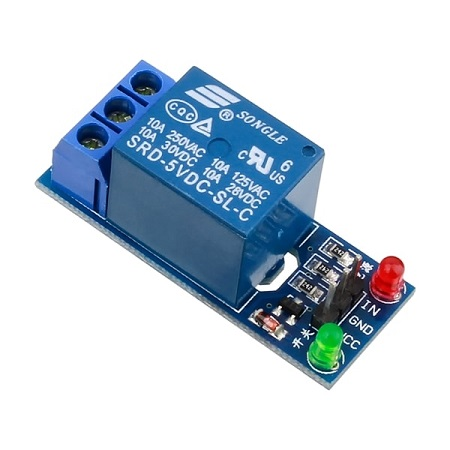
\includegraphics[width=1.75in]{relay.jpg} \\
            \caption{Single channel relay}
            \label{fig:relay} 
        \end{figure}
    Electromechanical switch used to control high-power devices with low-power signals. Enables the isolation between low-voltage circuits and high-voltage circuits, ensuring safety in control systems.
    
    \item \textbf{Breadboard}\\
    \begin{figure}[H]
            \centering
            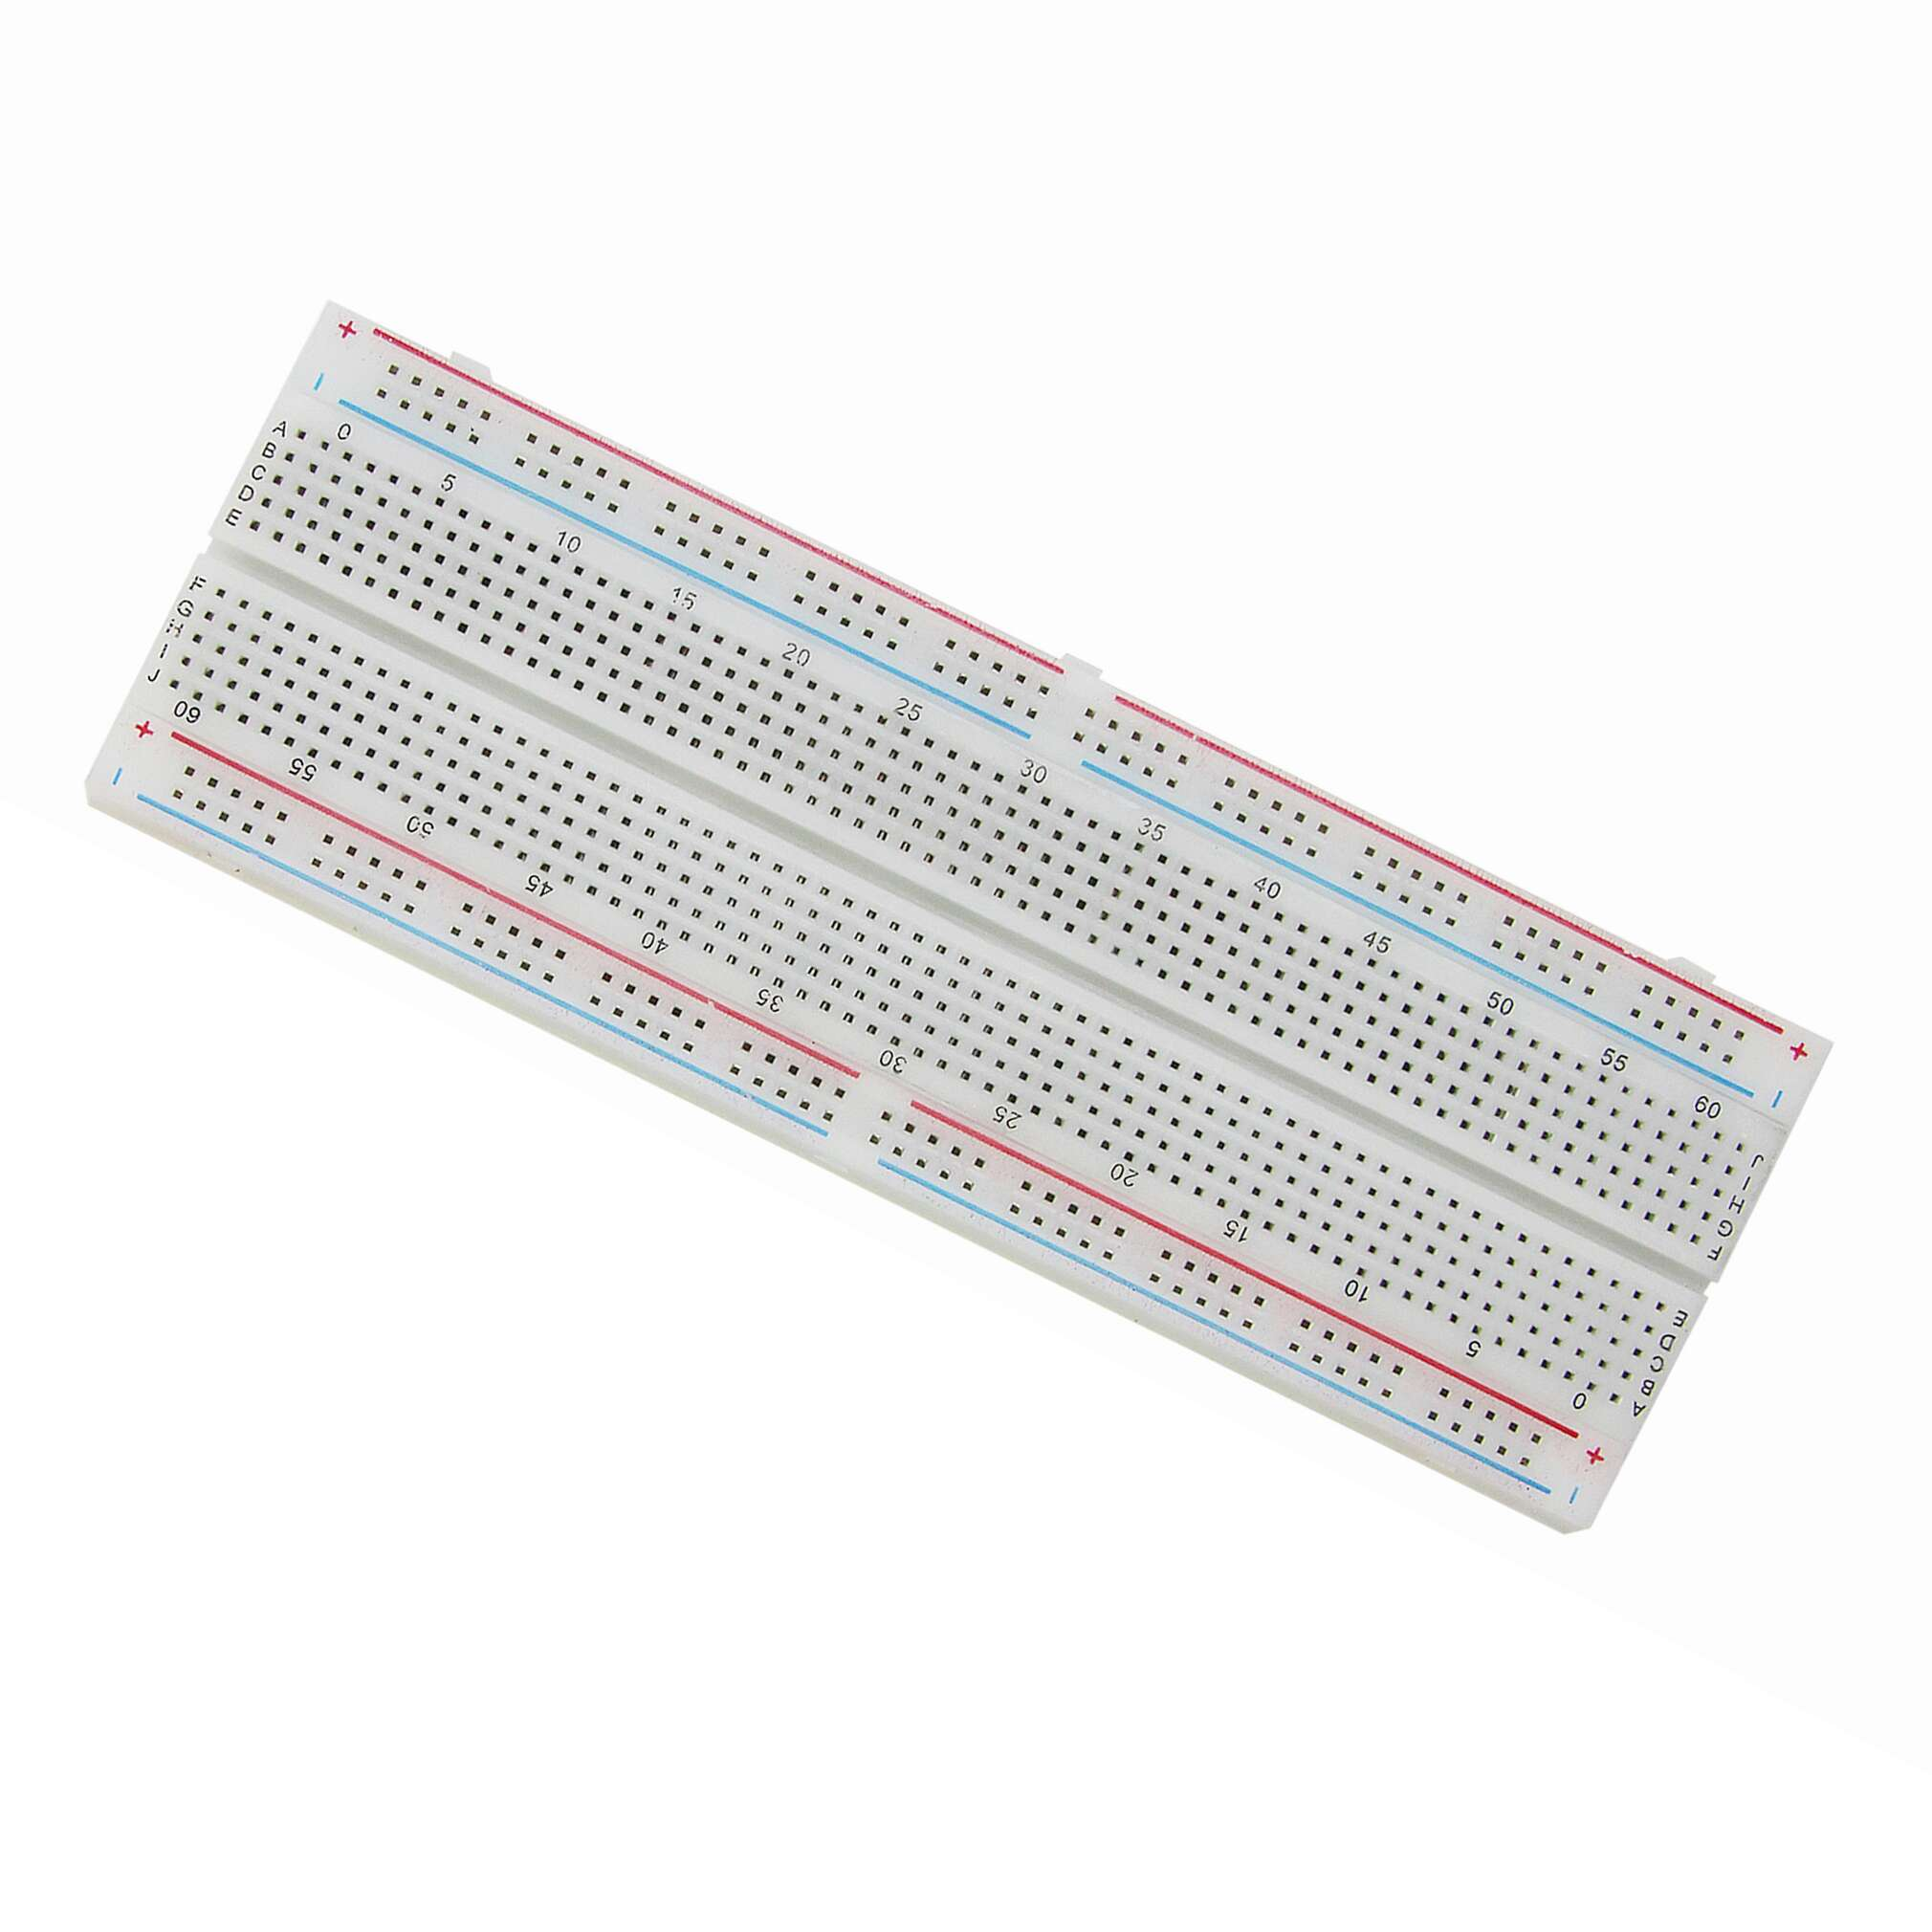
\includegraphics[width=1.75in]{breadboard.jpg} \\
            \caption{Breadboard}
            \label{fig:breadboard} 
        \end{figure}
    Prototyping tool for electronics projects, allowing components to be easily connected and tested without soldering. Ideal for rapid prototyping and experimenting with circuit designs.
    
    \item \textbf{Resistors}\\
    \begin{figure}[H]
            \centering
            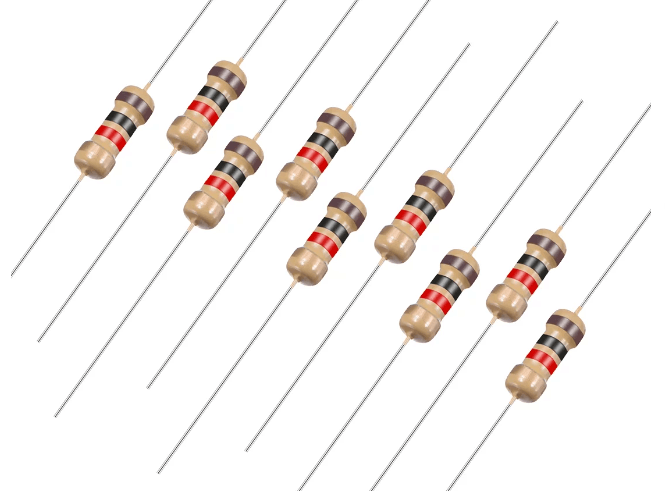
\includegraphics[width=1.75in]{resistors.png} \\
            \caption{Resistors}
            \label{fig:resistors} 
        \end{figure}
    A resistor is a passive electronic component used in IoT devices to limit current, divide voltages, or protect other components from excessive current flow. Resistors are critical for ensuring the safe and efficient operation of IoT circuits.
    
    \item \textbf{NPN Transistors}\\
    \begin{figure}[H]
            \centering
            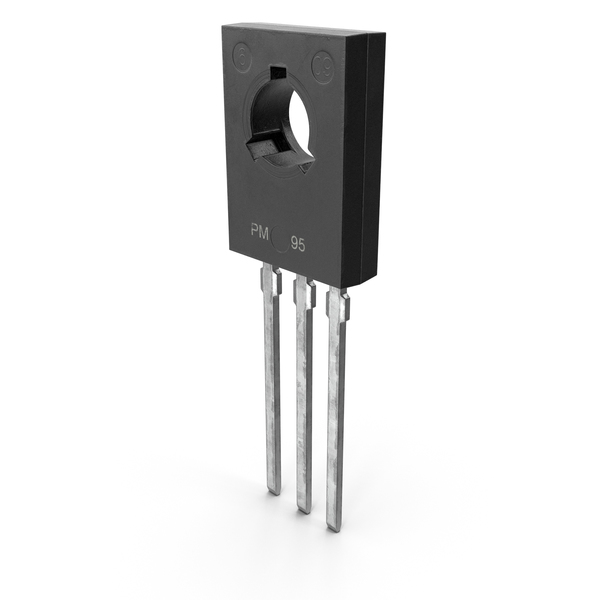
\includegraphics[width=1.75in]{transistors.jpg} \\
            \caption{NPN-Transistor}
            \label{fig:transistor} 
        \end{figure}
    An NPN transistor is commonly used as a switch or amplifier for controlling electronic signals in circuits. The NPN transistor consists of three layers of semiconductor material: n-type (negative), p-type (positive), and another n-type (negative), which are arranged as Emitter (E), Base (B), and Collector (C).
\end{enumerate}
    
    
